\documentclass{article}
\usepackage[margin=24mm]{geometry}
\usepackage{tikz}
\title{Composed inverse functions in the network search}
\date{Created-at: 2026-10-30 02:18 +01:00}
\begin{document}\maketitle
\paragraph{Goal.} Continue the working norm-network loop with the actual
norm--inverse--product--cleanup dependencies. Reuse the existing reverse-jet
callsite map and883-qubit incumbent. First discriminate whether exact composed
Boolean functions expose useful sharing that separate quadratic blocks hide.
Then lower admissible shared-function alternatives, verify their phase/cleanup,
and screen them using the existing global live-register envelope. No gain is
promised before measurement.
\paragraph{Ownership.} Core retains the authored typed function/operation model.
Graph supplies exact binary bases and reconstruction witnesses through its
existing example/facade; no consumer rank solver. Quantum owns bounded Boolean
coefficient evaluation, circuit lifetime lowering and phase contracts. Pgraph
MSG/SSG remains the network generator. The native adapter and HermiteLibrary own
binding to unchanged source-bound public runtime and native field verification.
\paragraph{Discriminating experiment.} At six input bits, enumerate all64
values and exact ANF coefficients of input bits, norm products, inverse-norm
bits and proposed products. Compare prefix and combined ranks and reconstruct
the requested inverse/zero flag. A basis change alone cannot lower a full-rank
space. A useful relation must remove an actual paid product after prefix costs,
cleanup and retained qubits are counted. Keep alternative prefixes and resulting
networks; no isolated long random-flip campaign.
\paragraph{Implementation scope.} Extend arithmetic.py/source vocabulary and
Quantum synthesis only where the experiment supports a valid lowering. Reuse
quadratic factor emission, exact basis verification and existing network feedback.
If explicit column weights are needed, extend only the Graph CLI adapter to its
existing binary-weighted-basis API, with source-bound costs; no provider solver
rewrite. Files: arithmetic.py, reversible.py, hermite.py as needed;
synthesis/arithmetic.rs, network.rs and a cohesive composed-function module if
required; source metadata/fixture, CLI, focused tests, quantum\_network.py,
existing report.py and README. Exact final list belongs in the report.
\paragraph{Verification.} Algebra certificates compare all64 inputs and every
reconstructed function, including zero. Small unitary XOR paths check all4096
input/target states. Fresh-output/measured cleanup must have an explicit separate
contract and phase proof. Native runs serialize/reload circuits and use independent
GF arithmetic, then cross-pair affected jet directions. Only an equivalent,
globally promising candidate receives the102400-shot official local verifier.
No local-block Q-squared-T improvement is reported as a whole-decoder result.
\paragraph{Caps and resources.} Preserve existing24-wire/12-data/512-gate
limits on the bounded primitive verifier; larger native jets retain their separate
limits. At most1600 proposed product columns,64 coefficient coordinates and
16 observed networks initially; no unbounded SSG. Native probe guard900s,
one CPU/2GiB for small kernels,12GiB/3600s only if full verification is justified.
Amaterasu has313GiB free and about19GiB available RAM. Expected60--100min for
model/certificate work, tests and native comparison; resource monitoring is a
guard, not an unsolicited speed benchmark. No GPU, WSL or source-tree copies.
\paragraph{Repository and risk.} Transformation feat/unversioned c90eb2b,
fresh fetch succeeds and upstream is current. Preserve unrelated changes.
Graph source is read-only unless the CLI weight adapter proves necessary; fetch
its remotes before edits. Existing uncommitted Graph API remains a recorded local
integration dependency. No new dependency or CORE.YAML-protected item is planned.
No commit/push/submission. Rollback only named task edits, keep prior kernels.
Worst case: composed rank gives no sharing, or retained cache loses at global
qubit peak; report that measured limit and do not promote the candidate.
\paragraph{Refinement,02:27.} The separated input-times-inverse family has
rank35 including a16-dimensional free prefix, so its full product span does
not contract. Include mixed prefix parities to test identities involving
cached norm products; at most57 operand forms give1596 pairs. This motivates
the1600 column cap above before the mixed-family implementation.
\paragraph{Refinement,02:34.} Minimizing a basis for the whole supplied span
does not minimize reconstruction of the seven requested outputs. Extend Graph's
binary matroid owner with bounded exact basis exchanges and a required-column
beam objective, retaining the already available prefix. This is a provider API,
not a consumer rank solver. Add direct reconstruction/certificate tests; cap
exchange evaluations at4096 and retain four states. The native gate search will
consume the resulting certificates through the same Core source identity.
\begin{center}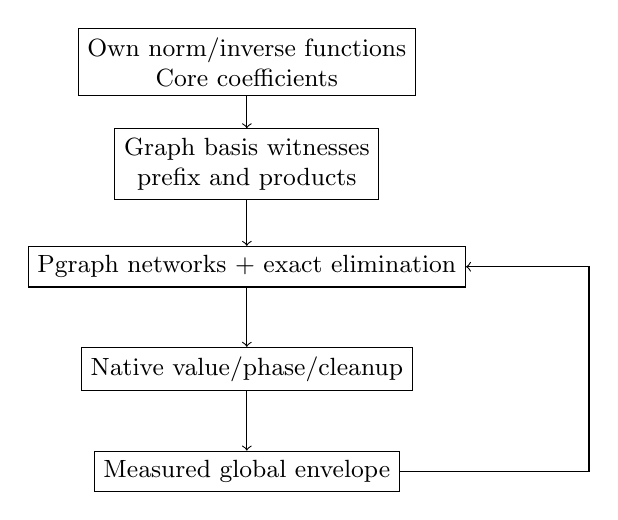
\begin{tikzpicture}[every node/.style={draw,align=center,font=\small},node distance=13mm]
\node (a) {Own norm/inverse functions\\Core coefficients};
\node (b) [below of=a] {Graph basis witnesses\\prefix and products};
\node (c) [below of=b] {Pgraph networks + exact elimination};
\node (d) [below of=c] {Native value/phase/cleanup};
\node (e) [below of=d] {Measured global envelope};
\draw[->] (a)--(b);\draw[->] (b)--(c);\draw[->] (c)--(d);\draw[->] (d)--(e);
\draw[->] (e.east)--++(24mm,0)|-(c.east);
\end{tikzpicture}
\end{center}
\end{document}
